% !TEX program = xelatex
\documentclass[10pt,letterpaper,twocolumn]{article}

\usepackage[top=0.75in,bottom=0.75in,left=0.75in,right=0.75in,footskip=12pt]{geometry}
\usepackage{fontspec}
\usepackage{unicode-math}
\setmainfont{Latin Modern Roman}[
  Extension=.otf,
  UprightFont=lmroman10-regular,
  BoldFont=lmroman10-bold,
  ItalicFont=lmroman10-italic,
  BoldItalicFont=lmroman10-bolditalic,
]
\setsansfont{Latin Modern Sans}[
  Extension=.otf,
  UprightFont=lmsans10-regular,
  BoldFont=lmsans10-bold,
  ItalicFont=lmsans10-oblique,
  BoldItalicFont=lmsans10-boldoblique,
]
\setmonofont{Latin Modern Mono}[
  Extension=.otf,
  UprightFont=lmmono10-regular,
  BoldFont=lmmonolt10-bold,
  ItalicFont=lmmono10-italic,
  Scale=0.85,
]
\newfontfamily\acbold{ywft-processing-bold}[
  Path=../../system/public/type/webfonts/,
  Extension=.ttf
]

\usepackage{xcolor}
\usepackage{titlesec}
\usepackage{enumitem}
\usepackage{booktabs}
\usepackage{tabularx}
\usepackage{fancyhdr}
\usepackage{hyperref}
\usepackage{xurl}
\usepackage{graphicx}
\graphicspath{{figures/}}
\usepackage{microtype}
\usepackage[font=footnotesize]{caption}
\usepackage{listings}
\usepackage{natbib}
\usepackage{tikz}
\usetikzlibrary{arrows.meta,calc,fit,positioning,shapes.geometric}
\usepackage[colorspec=0.92]{draftwatermark}

\definecolor{acpink}{RGB}{180,72,135}
\definecolor{acpurple}{RGB}{120,80,180}
\definecolor{acdark}{RGB}{64,56,74}
\definecolor{acgray}{RGB}{119,119,119}
\definecolor{acblue}{RGB}{42,100,212}
\definecolor{acgreen}{RGB}{42,154,58}
\definecolor{acorange}{RGB}{216,120,0}
\definecolor{papercream}{RGB}{250,246,235}
\definecolor{klbg}{RGB}{250,248,252}

\DraftwatermarkOptions{
  text=WORKING DRAFT,
  fontsize=3cm,
  color=acpink!18,
  angle=45,
  pos={0.5\paperwidth,0.5\paperheight}
}

\hypersetup{
  colorlinks=true,
  linkcolor=acpurple,
  urlcolor=acpurple,
  citecolor=acpurple,
  pdfauthor={@jeffrey},
  pdftitle={Equal Enough to Draw: Homotopy Type Theory as a Design Lens for KidLisp},
}

\titleformat{\section}{\normalfont\bfseries\normalsize\uppercase}{\thesection.}{0.5em}{}
\titlespacing{\section}{0pt}{1.2em}{0.3em}
\titleformat{\subsection}{\normalfont\bfseries\small}{\thesubsection}{0.5em}{}
\titlespacing{\subsection}{0pt}{0.8em}{0.2em}

\pagestyle{fancy}
\fancyhf{}
\renewcommand{\headrulewidth}{0pt}
\fancyhead[C]{\footnotesize\color{acpink}\textit{Working Draft --- not for citation}}
\fancyfoot[C]{\footnotesize\thepage}

\lstdefinelanguage{kidlisp}{
  morekeywords=[1]{def,if,repeat,once,later,die},
  morekeywords=[2]{wipe,ink,line,box,circle,plot,flood,write,paste,embed},
  morekeywords=[3]{scroll,zoom,spin,blur,contrast,suck,bake,burn},
  morekeywords=[4]{random,wiggle,sin,cos,min,max,mod},
  sensitive=true,
  morecomment=[l]{;},
  morestring=[b]",
}
\lstdefinestyle{kidlispstyle}{
  language=kidlisp,
  basicstyle=\ttfamily\small,
  keywordstyle=[1]\color{acpurple}\bfseries,
  keywordstyle=[2]\color{acblue}\bfseries,
  keywordstyle=[3]\color{acpink},
  keywordstyle=[4]\color{acgreen},
  commentstyle=\color{acgray}\itshape,
  stringstyle=\color{acorange},
  breaklines=true,
  columns=fullflexible,
  frame=single,
  rulecolor=\color{acgray!30},
  backgroundcolor=\color{klbg},
  xleftmargin=0.5em,
  xrightmargin=0.5em,
  aboveskip=0.5em,
  belowskip=0.5em,
  showstringspaces=false,
}
\lstset{style=kidlispstyle}

\tikzset{
  point/.style={circle,draw=acdark,fill=white,minimum size=5.5mm,inner sep=0pt,font=\scriptsize\bfseries},
  layer/.style={rounded corners=2pt,draw=acgray!60,fill=white,inner sep=5pt,font=\footnotesize,align=center},
  evidence/.style={rounded corners=2pt,draw=acpurple!70,fill=acpurple!8,inner sep=5pt,font=\footnotesize,align=center},
  runtime/.style={rounded corners=2pt,draw=acpink!75,fill=acpink!8,inner sep=5pt,font=\footnotesize,align=center},
  arr/.style={-{Latex[length=2mm]},line width=0.55pt,draw=acdark!80},
  pathline/.style={-{Latex[length=2mm]},line width=1.2pt,draw=acpink},
}

\newcommand{\acdot}{{\color{acpink}.}}
\newcommand{\ac}{Aesthetic{\acdot}Computer}
\newcommand{\kl}{\textsf{KidLisp}}
\newcommand{\code}[1]{\texttt{\detokenize{#1}}}
\newcommand{\judges}[3]{#1\;\vdash\;#2:#3}
\newcommand{\claim}[1]{\textsf{#1}}

\setlist[itemize]{nosep,leftmargin=1.2em,itemsep=0.1em}
\setlist[enumerate]{nosep,leftmargin=1.2em,itemsep=0.1em}
\setlength{\columnsep}{1.8em}
\setlength{\parindent}{1em}
\setlength{\parskip}{0.3em}
\tolerance=800
\emergencystretch=1em
\hyphenpenalty=50
\raggedbottom

\InputIfFileExists{version}{}{\providecommand{\paperhash}{dev}\providecommand{\paperrev}{?}}
\InputIfFileExists{history}{}{\providecommand{\paperhistory}{}}

\begin{document}

\twocolumn[{%
\begin{center}
{\acbold\fontsize{26pt}{30pt}\selectfont\color{acdark} Equal Enough to Draw}\par
\vspace{0.45em}

\includegraphics[width=0.62\textwidth]{cover}\par
\vspace{0.35em}
{\itshape\fontsize{13pt}{16pt}\selectfont\color{acpink} Homotopy Type Theory as a Design Lens for KidLisp}\par
\vspace{0.5em}
{\small\color{acgray}\href{https://prompt.ac/@jeffrey}{@jeffrey} \,\(\cdot\)\, Aesthetic{\acdot}Computer \,\(\cdot\)\, ORCID \href{https://orcid.org/0009-0007-4460-4913}{0009-0007-4460-4913}}\par
\vspace{0.45em}
{\footnotesize\sffamily\color{acpink}\textbf{EN}\quad\color{acgray} DA \quad ES \quad ZH \quad JA \quad RU}\par
\vspace{0.5em}
{\color{acpink}\rule{\textwidth}{1.2pt}}
\vspace{0.45em}
\end{center}

\begin{quote}
\small\noindent\textbf{Abstract.}
Homotopy type theory treats identity as structured evidence: points may be joined by paths, paths by higher paths, and equivalent types may be identified through univalence. \kl{} is almost the opposite kind of object --- an untyped, effectful, frame-by-frame Lisp for drawing, sound, timing, and composition inside \ac{}. This study asks what the first can honestly teach the second. I separate source equality, normalized-AST equality, render equality, trace equality, and contextual substitutability; define a bounded observational relation indexed by host, input trace, frame horizon, and tolerance; and use it to design a proof-carrying companion layer for KidLisp. The proposal does not claim that current KidLisp implements dependent types, higher inductive types, or univalence. It uses HoTT to expose where the runtime currently says ``same'' without saying why. A tiny art language does not need a theorem prover in its prompt. It does need better witnesses when one piece is allowed to stand in for another.
\end{quote}
\vspace{0.45em}
}]

\section{Two Circles}
\label{sec:intro}

These two KidLisp fragments can draw the same circle:

\begin{lstlisting}
black
(ink pink)
(circle w/2 h/2 20)
\end{lstlisting}

\begin{lstlisting}
black
(def radius 20)
(ink pink)
(circle (/ w 2) (/ h 2) radius)
\end{lstlisting}

They are not the same text. Their parsed trees differ. One adds a name to the evaluator's definition environment. On a particular host, canvas size, input trace, random seed, and frame, their pixel buffers may agree exactly. Put either inside a larger piece and the agreement can disappear: the second fragment occupies a global name, costs different work, and may interact with later code. ``They draw the same circle'' is true only after the sentence supplies its missing conditions.

That ordinary example is the opening for homotopy type theory (HoTT). In intensional type theory, equality is not merely a Boolean test performed after the fact. An identity type can itself contain terms --- evidence that one thing is identified with another~\citep{martinlof1984,hottbook2013}. Under the homotopical reading, a type is a space, its terms are points, identities are paths, and identities between identities are higher paths~\citep{awodey2009,hottbook2013}. The geometry is not decoration. It records that there may be more than one way to establish sameness, and those ways may themselves agree or disagree.

KidLisp descends from a different economy. Lisp gives it compact symbolic trees~\citep{mccarthy1960recursive}; creative-coding systems give it immediate graphics, animation, and a tight edit--run loop~\citep{mccarthy2015p5,jack2026hydra,scudder2026kidlisp}. Its job is to make a picture happen now. HoTT's job is not to make pictures. The productive encounter is therefore not ``add HoTT syntax to KidLisp.'' It is to ask which identities a live art language already relies on, which evidence it throws away, and where explicit paths could make refactoring, porting, remixing, and preservation safer.

The study proceeds in four moves. Section~\ref{sec:hott} gives the minimum HoTT needed for the comparison. Section~\ref{sec:runtime} reads the actual KidLisp evaluator. Sections~\ref{sec:relation} and~\ref{sec:translation} define a bounded observational relation and mark the limits of the analogy. Sections~\ref{sec:design}--\ref{sec:limits} turn the result into a narrow tooling proposal, then argue against importing a proof assistant into the live language.

\section{Identity Has Levels}
\label{sec:hott}

The familiar programming-language distinction between definitional and propositional equality is already enough to improve the conversation. \emph{Definitional} equality is computation the checker can see directly: two expressions reduce to the same form. \emph{Propositional} equality is inhabited by a term that witnesses identity. HoTT keeps the latter structure instead of forcing all equality proofs to be indistinguishable.

\begin{figure*}[t]
\centering
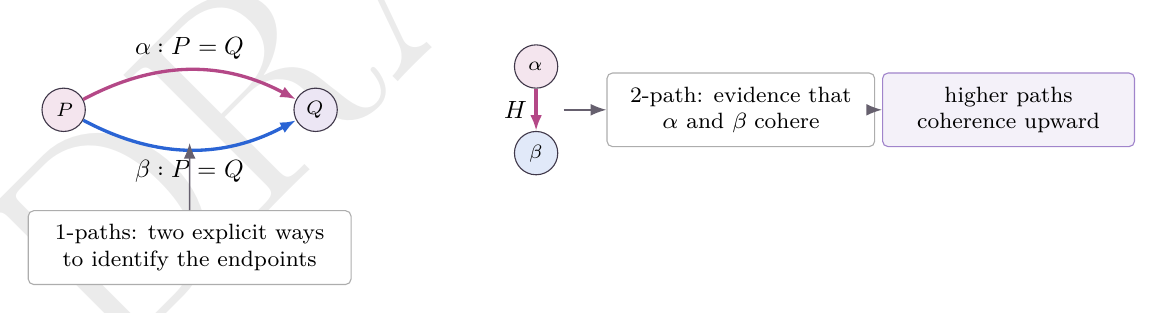
\begin{tikzpicture}[x=1cm,y=1cm]
  \node[point,fill=acpink!14] (p) at (0,0) {$P$};
  \node[point,fill=acpurple!14] (q) at (3.2,0) {$Q$};
  \draw[pathline,bend left=28] (p) to node[above,font=\small] {$\alpha:P=Q$} (q);
  \draw[pathline,bend right=28,draw=acblue] (p) to node[below,font=\small] {$\beta:P=Q$} (q);
  \node[layer,minimum width=4.1cm] (one) at (1.6,-1.75) {1-paths: two explicit ways\\to identify the endpoints};
  \draw[arr] (one.north) -- ($(p)!0.5!(q)+(0,-0.42)$);

  \node[point,fill=acpink!14] (a) at (6.0,0.55) {$\alpha$};
  \node[point,fill=acblue!14] (b) at (6.0,-0.55) {$\beta$};
  \draw[pathline] (a) -- node[left,font=\small] {$H$} (b);
  \node[layer,minimum width=3.4cm] (two) at (8.6,0) {2-path: evidence that\\$\alpha$ and $\beta$ cohere};
  \draw[arr] (6.35,0) -- (two.west);

  \node[evidence,minimum width=3.2cm] (higher) at (12.0,0) {higher paths\\coherence upward};
  \draw[arr] (two.east) -- (higher.west);
\end{tikzpicture}
\caption{The identity ladder used in this study. $P$ and $Q$ are endpoints; $\alpha$ and $\beta$ are distinct witnesses that identify them; $H$ identifies those witnesses. For KidLisp the picture is initially a design vocabulary, not a constructed HoTT model: source rewrites and render tests do not automatically satisfy the laws required of path types.}
\label{fig:identity-ladder}
\end{figure*}

Three HoTT ideas matter here.

\textbf{Paths carry method.} A path says not only that endpoints coincide but how the identification is obtained. Composition and inversion let paths form the beginnings of groupoid structure. Computational higher type theories make that structure executable through interval variables, coercion, and Kan operations~\citep{angiuli2016higher,cohen2017cubical}.

\textbf{Higher inductive types add path constructors.} Ordinary inductive types specify point constructors. Higher inductive types may also specify paths and higher paths, supporting spaces, quotients, truncations, and pushouts inside type theory~\citep{sojakova2015hits,lumsdaine2020hits}. A tempting KidLisp reading is ``pieces plus declared equivalences.'' Tempting is not sufficient. A valid higher inductive presentation needs elimination and computation principles, not a folder of screenshots that look alike.

\textbf{Univalence turns equivalence into identity.} Roughly, the univalence principle identifies the identity of types with equivalence between them~\citep{hottbook2013}. Cubical type theories supply computational accounts of this principle~\citep{cohen2017cubical}. Univalence is not the slogan ``similar outputs are equal.'' It applies to equivalences with enough structure to support transport. That demand --- what can safely be transported? --- is the sharpest question HoTT contributes to KidLisp.

The resulting ladder is shown in Figure~\ref{fig:identity-ladder}. Formal developments use this structure for substantial machine-checked mathematics~\citep{hou2016blakers}; parametricity results can even derive homotopical consequences from polymorphic terms~\citep{uemura2017homotopies}. This paper stays much lower. It uses the ladder to keep four claims from collapsing into one word.

\section{What KidLisp Actually Does}
\label{sec:runtime}

The current reference implementation is a large JavaScript tree-walking evaluator at \path{system/public/aesthetic.computer/lib/kidlisp.mjs}. The parser tokenizes S-expressions, drops comments and commas, converts numeric atoms, and automatically appends closing parentheses when input is incomplete. Before execution it expands some compact arithmetic forms and recognizes timing tokens. A program is therefore already interpreted through a forgiving normalization boundary: source strings that differ can become the same or closely related abstract syntax tree.

Every paint cycle evaluates the stored AST against a host API. The environment mixes several kinds of state:

\begin{itemize}
\item \code{globalDef} and local loop bindings for names;
\item frame, clock, timing triggers, \code{once} records, and deterministic or host-fed signals;
\item drawing state and offscreen buffers;
\item embedded \code{$code} programs fetched through caches and rendered as layers;
\item post-composite transforms such as zoom, scroll, contrast, and brightness.
\end{itemize}

The \code{repeat} form enforces a numeric count and a 10,000-iteration safety ceiling, then may enter specialized drawing fast paths. The \code{def} form mutates a definition environment. \code{once} hashes the body to decide whether it has run. Embedded pieces can load asynchronously and introduce their own buffers. The 2026 Decree names portable host obligations --- Core, Render, and Audio conformance --- but several semantic details remain draft work~\citep{scudder2026decree}.

This is a productive creative runtime. It is not a dependent type theory. It has no universe hierarchy, identity eliminator, path type, proof terms, higher inductive declarations, or type checker. It is neither pure nor total; its output depends on host capabilities, time, input, cached programs, and mutable rendering state. Calling its AST nodes ``points in a space'' does not repair any of that.

The runtime nevertheless has an identity problem. A stored \texttt{\$code} may move between JavaScript, Common Lisp, WASM, or a future Swift implementation. A refactor may take an optimized path. A published piece may embed a child by content address while the host changes beneath both. The system must repeatedly decide whether the thing after the move is still the same piece. Today that decision is distributed across source IDs, caches, conformance prose, and visual comparison. HoTT makes the missing evidence visible.

\section{Bounded Observational Equality}
\label{sec:relation}

Let $R_H(P,I,n)$ be the observable output of program $P$ on host profile $H$, under input trace $I$, at frame $n$. The observation can contain a pixel buffer, audio samples, emitted navigation actions, logs, and declared resource accesses. For a distance $d$ on observations, define

\begin{align*}
 P &\approx_{H,I,N,\varepsilon} Q \\
 &\Longleftrightarrow
 \max_{0\leq n<N} d\!\left(R_H(P,I,n),R_H(Q,I,n)\right)\leq\varepsilon.
\end{align*}

This is a testable relation. It is indexed because omitting the indices makes the claim false or meaningless. Exact pixels on one 128-by-128 canvas do not establish equality on a different resolution. Silence in a two-second trace does not establish equality after the third second. A deterministic pointer trace says nothing about a microphone. A tolerance of one channel value is not exact equality.

The relation has useful algebra, but not for free. Reflexivity holds when observation itself is deterministic. Symmetry follows from a symmetric distance. Transitivity at a fixed tolerance generally fails: if $P$ differs from $Q$ by $\varepsilon$ and $Q$ from $S$ by $\varepsilon$, the triangle inequality gives $2\varepsilon$, not $\varepsilon$. Host nondeterminism, network fetches, clocks, and floating-point differences complicate even those statements.

This is why I call each result a \emph{certificate}, not a proof of HoTT identity. A certificate records a bounded experiment and the claim it supports. It can be composed only by rules that preserve its indices and error budget.

\begin{table*}[t]
\centering
\small
\begin{tabularx}{\textwidth}{@{}p{0.18\textwidth}p{0.27\textwidth}p{0.25\textwidth}X@{}}
\toprule
Identity claim & Evidence & Safe transport & Counterexample \\
\midrule
Source identity & byte-for-byte source hash & attribution, exact archival retrieval & same AST after whitespace or auto-closing \\
Normalized-AST identity & canonical parsed tree & syntax-directed analyses & evaluator or host version changes meaning \\
Frame equality & pixel/audio diff at frame $n$ & that observation only & timing diverges on frame $n+1$ \\
Trace equality & bounded diff over $N$ frames and input trace $I$ & replay under recorded indices & unseen input, larger horizon, another host \\
Contextual equivalence & quantified preservation in allowed contexts & substitution inside those contexts & global names, timing, I/O, performance \\
Type equivalence & functions with inverse laws and coherence & dependent data via transport & matching screenshots alone \\
\bottomrule
\end{tabularx}
\caption{Six meanings of ``same'' that a KidLisp tool should keep separate. Each row supports different transport. The final row is the one univalence speaks to; the middle rows are engineering evidence, not substitutes for it.}
\label{tab:identity-claims}
\end{table*}

Table~\ref{tab:identity-claims} is the practical result. The first four rows can be implemented now. Contextual and type equivalence require a semantics strong enough to quantify beyond finite render traces. The table prevents the system from promoting evidence merely because the word \emph{equivalent} sounds mathematical.

\section{A Translation With Red Lines}
\label{sec:translation}

There is a fruitful correspondence between the two domains, provided every arrow is labeled ``design analogy'' until formalized.

\subsection{Programs as points}

A normalized KidLisp AST can be treated as a point in a set of programs. A richer behavior space can index that point by host profile, inputs, and observation semantics. This is ordinary mathematical modeling. It does not make the set an $\infty$-groupoid.

\subsection{Refactorings as paths}

A source-to-source transformation can carry its derivation: expand \code{w/2} into \code{(/ w 2)}, alpha-rename a local iterator, replace a primitive with a decree-certified equivalent, or inline a definition when no capture occurs. Such a derivation resembles a path because it has endpoints, composes, and may be reversible.

Some transformations are not reversible. Constant folding loses syntax; dead-code elimination forgets an unreachable branch; render-only certification forgets internal state. Those are directed rewrites, not HoTT paths. Work on synthetic $\infty$-categories distinguishes directed morphisms from invertible paths for exactly this kind of reason~\citep{riehl2017synthetic}. The paper's first red line is therefore: \emph{do not draw an arrow with two heads unless the tool can run both ways or provide inverse evidence.}

\subsection{Rewrite coherence as higher paths}

Suppose one tool rewrites $P$ to $Q$ by expanding arithmetic first and renaming second, while another does those steps in the opposite order. A commuting-square check can witness that the two routes reach the same normalized AST. That witness is a credible 2-dimensional object. A pair of video diffs that merely happen to pass is weaker: it establishes two bounded observations, not coherence between transformations.

\subsection{Portable hosts and transport}

The most valuable application is host portability. The Decree already states a shared ABI and conformance levels. A stronger conformance artifact could define an equivalence between two host interpretations for a fragment $F$ of the language. Then a property established for a piece in $F$ --- bounds safety, absence of unsupported calls, a deterministic render trace --- could be transported across the host equivalence. This begins to rhyme with univalence because structured equivalence justifies substitution. It remains an engineering theorem about a specified fragment, not the univalence axiom itself.

\subsection{Quotients and higher inductive types}

One can imagine a type of pieces generated by syntax points and certified path constructors:

\[
\begin{array}{ll}
\mathsf{code} &: \mathsf{AST}\to\mathsf{Piece},\\
\mathsf{rename} &: \mathsf{code}(P)=\mathsf{code}(\alpha(P)),\\
\mathsf{hostEq} &: \mathsf{Conforms}(H_1,H_2,F)\\
 &\qquad\to \mathsf{render}_{H_1}(P)=\mathsf{render}_{H_2}(P).
\end{array}
\]

That is a useful research sketch. To become a higher inductive type it would need precise formation, introduction, elimination, and computation rules, plus a formal semantics for the effects the runtime exposes. The paper's second red line is: \emph{a quotient-style UI is not a higher inductive type until its eliminators are known.}

\section{The Companion Layer}
\label{sec:design}

The proposal leaves KidLisp source alone. The prompt remains a place to write \code{(circle ? ? ?)} and see something happen. Evidence lives beside the piece in three layers (Figure~\ref{fig:companion}).

\begin{figure*}[t]
\centering
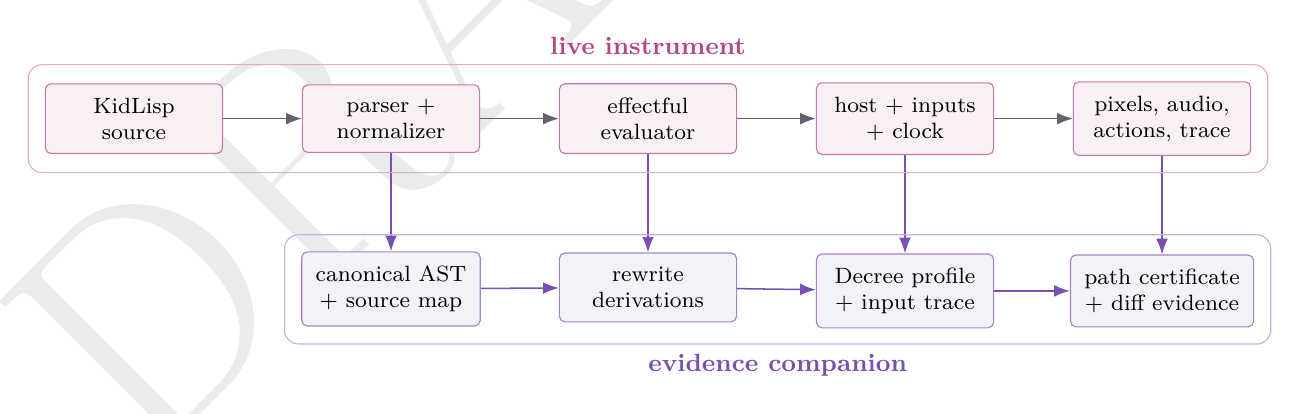
\begin{tikzpicture}[node distance=8mm and 10mm]
  \node[runtime,minimum width=2.25cm] (source) {KidLisp\\source};
  \node[runtime,minimum width=2.25cm,right=of source] (parser) {parser +\\normalizer};
  \node[runtime,minimum width=2.25cm,right=of parser] (eval) {effectful\\evaluator};
  \node[runtime,minimum width=2.25cm,right=of eval] (host) {host + inputs\\+ clock};
  \node[runtime,minimum width=2.25cm,right=of host] (obs) {pixels, audio,\\actions, trace};
  \draw[arr] (source) -- (parser);
  \draw[arr] (parser) -- (eval);
  \draw[arr] (eval) -- (host);
  \draw[arr] (host) -- (obs);

  \node[evidence,minimum width=2.25cm,below=1.25cm of parser] (norm) {canonical AST\\+ source map};
  \node[evidence,minimum width=2.25cm,below=1.25cm of eval] (claims) {rewrite\\derivations};
  \node[evidence,minimum width=2.25cm,below=1.25cm of host] (profile) {Decree profile\\+ input trace};
  \node[evidence,minimum width=2.25cm,below=1.25cm of obs] (cert) {path certificate\\+ diff evidence};
  \draw[arr,draw=acpurple] (parser) -- (norm);
  \draw[arr,draw=acpurple] (eval) -- (claims);
  \draw[arr,draw=acpurple] (host) -- (profile);
  \draw[arr,draw=acpurple] (obs) -- (cert);
  \draw[arr,draw=acpurple] (norm) -- (claims);
  \draw[arr,draw=acpurple] (claims) -- (profile);
  \draw[arr,draw=acpurple] (profile) -- (cert);

  \node[fit=(source)(obs),draw=acpink!45,rounded corners=5pt,inner sep=6pt,label={[font=\small\bfseries,text=acpink]above:live instrument}] {};
  \node[fit=(norm)(cert),draw=acpurple!45,rounded corners=5pt,inner sep=6pt,label={[font=\small\bfseries,text=acpurple]below:evidence companion}] {};
\end{tikzpicture}
\caption{The proposed architecture. The live instrument remains permissive and immediate. A companion lane records normalization, rewrite derivations, host and input indices, observations, and bounded equivalence certificates. The two lanes meet at explicit taps; the checker never has to sit inside the paint loop.}
\label{fig:companion}
\end{figure*}

\textbf{1. Canonicalization.} The parser emits a versioned normalized AST while preserving a source map. Harmless surface differences can then receive definitional treatment without destroying the exact published source. Canonicalization must be versioned because the current parser's auto-closing and macro expansion are semantic choices.

\textbf{2. Tracing.} The evaluator emits an observation trace: host/decree version, dimensions, random seed, clock mode, input events, embedded-content hashes, API calls, output hashes, and optional full buffers. The trace turns a visual hunch into a replayable claim.

\textbf{3. Checking.} An offline checker compares endpoints and writes a certificate. A minimal form could be:

\begin{lstlisting}[language={},basicstyle=\ttfamily\scriptsize]
{
  "from": "sha256:...",
  "to": "sha256:...",
  "claim": "trace-equivalent",
  "profile": "KDL-26 Core+Render",
  "canvas": [128, 128],
  "frames": 240,
  "inputTrace": "sha256:...",
  "rgbaMax": 0,
  "embedded": ["$39i@sha256:..."]
}
\end{lstlisting}

The certificate is content-addressed, reviewable, and invalidated when an endpoint, embedded child, checker version, or host profile changes. It can support a green ``same render under this trace'' badge without claiming universal program equivalence.

\subsection{Four useful judgments}

The checker can expose four statements in increasing strength:

\begin{enumerate}
\item $\judges{v}{P\equiv Q}{\claim{normalized}}$ --- canonical ASTs coincide under normalizer version $v$.
\item $\judges{\rho}{P\rightsquigarrow Q}{\claim{derived}}$ --- rewrite derivation $\rho$ checks.
\item $\judges{H,I,N,\varepsilon}{P\approx Q}{\claim{observed}}$ --- bounded traces satisfy the metric.
\item $\judges{F}{H_1\simeq H_2}{\claim{conformant}}$ --- hosts agree for a declared language fragment $F$ under a separate conformance suite.
\end{enumerate}

Only the first is a candidate for definitional equality. The middle two carry explicit evidence. The fourth could eventually justify transport of results between hosts. Keeping the badges distinct is more important than making any badge sound impressive.

\section{Worked Cases}
\label{sec:cases}

\subsection{Centering arithmetic}

The opening programs offer the smallest certificate. A normalizer can expand \code{w/2} to \code{(/ w 2)}. It cannot erase \code{def radius} without proving that the binding is fresh, evaluates to 20, and is not later observed. If those side conditions are discharged, the tool has a derived rewrite. Otherwise it may still produce a bounded render certificate. The distinction says exactly what is known.

\subsection{Fast paths}

The evaluator recognizes common \code{repeat} drawing shapes and executes optimized paths. The optimized and generic evaluators should be connected by a conformance claim over the accepted fragment. Frame diffs are a start. A stronger account would give both routes the same small-step or denotational semantics and prove preservation. Until then, every optimization certificate should name its expression class, numeric domain, canvas bounds, and host arithmetic.

\subsection{Embedded pieces}

A parent that calls \code{$39i} does not identify a child solely by a short public code. The observation depends on the resolved child source, cache state, dimensions, timing, alpha composition, and host. A valid parent certificate therefore closes over content hashes for its transitive embed tree. This resembles dependency transport more than function extensionality. The path is only as stable as its endpoints.

\subsection{Porting the Decree}

Suppose the JavaScript and Common Lisp hosts both claim \claim{Core+Render}. A corpus of reference pieces and frame comparisons can issue bounded host certificates. These do not establish full equivalence between implementations, but they can support a statement such as: ``for fragment $F$, canvas sizes $S$, traces $T$, and tolerance $\varepsilon$, the two hosts agree.'' That statement is honest, useful, and refinable. The route to stronger transport is to shrink ambiguity in the Decree, not to rename the corpus a proof.

\section{What This Buys the Artist}
\label{sec:artist}

Proof language can sound like maintenance language wearing a robe. The benefit has to reach the person drawing.

First, remix can preserve lineage at the level that matters. A fork may announce ``same trace, different source,'' ``same normalized piece,'' or ``new behavior.'' Second, optimization can stop being an invisible substitution. A fast path can carry the exact region over which it has been checked. Third, ports can report where fidelity ends: graphics match, audio is approximate, microphone behavior is untested. Fourth, archives can keep executable evidence beside code, so a future runtime knows what it is trying to preserve.

There is an aesthetic gain too. Multiple paths between pieces are not noise to collapse. One route may be pedagogical, one fast, one legible on a card, one tuned for a Game Boy. If two routes are certified to meet, the system can keep both. HoTT's best gift here is permission to treat sameness as structured plurality rather than forced deduplication.

\begin{figure}[t]
\centering
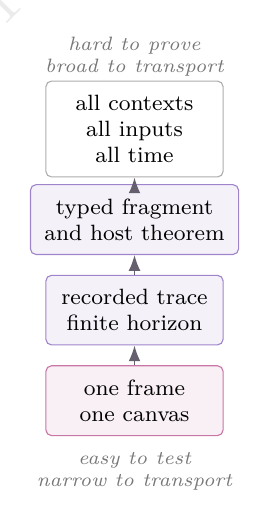
\begin{tikzpicture}[x=1cm,y=1cm]
  \node[layer,minimum width=2.25cm] (univ) at (0,2.7) {all contexts\\all inputs\\all time};
  \node[evidence,minimum width=2.25cm] (frag) at (0,1.55) {typed fragment\\and host theorem};
  \node[evidence,minimum width=2.25cm] (trace) at (0,0.4) {recorded trace\\finite horizon};
  \node[runtime,minimum width=2.25cm] (frame) at (0,-0.75) {one frame\\one canvas};
  \draw[arr] (frame) -- (trace);
  \draw[arr] (trace) -- (frag);
  \draw[arr] (frag) -- (univ);
  \node[font=\scriptsize\itshape,text=acgray,align=center] at (0,-1.65) {easy to test\\narrow to transport};
  \node[font=\scriptsize\itshape,text=acgray,align=center] at (0,3.62) {hard to prove\\broad to transport};
\end{tikzpicture}
\caption{The evidence ladder. Current render diffs live near the bottom. HoTT-level identity and univalent transport live near the top. A responsible tool shows the rung it reached instead of borrowing the name of a higher one.}
\label{fig:evidence-ladder}
\end{figure}

\section{Limits and Counter-Cases}
\label{sec:limits}

The central analogy can fail in several ways.

\textbf{Visual equality is too weak.} Two pieces can emit identical pixels while differing in audio, network activity, accessibility text, performance, energy use, or future state. Any observation algebra privileges what it measures.

\textbf{Finite testing is not contextual equivalence.} No practical trace corpus quantifies over every input and embedding context. Certificates must remain bounded and revocable.

\textbf{Effects resist path inversion.} A navigation action, network post, or destructive buffer operation cannot generally be undone. Directed type theory or effect semantics may be a better mathematical guide than HoTT for those portions of the runtime.

\textbf{Proof burden can kill immediacy.} KidLisp works because malformed parentheses close themselves and the canvas responds. Requiring proof obligations in the prompt would turn a tiny score into homework. The companion must remain optional during play and strict only at boundaries where substitution is being claimed: publishing a portable artifact, accepting an optimization, or declaring host conformance.

\textbf{Univalence is easy to misuse.} A pixel diff is not an equivalence of types. A pair of conversion functions without inverse and coherence laws is not enough. This paper offers a design program, not a model of KidLisp in cubical sets.

The hardest counter-case is artistic difference itself. A one-pixel discrepancy may be a bug in a conformance test or the entire point of a piece. No metric decides that for the artist. Certificates should describe evidence and leave aesthetic identity open.

\section{Research Program}
\label{sec:future}

A credible next study can proceed without changing KidLisp syntax:

\begin{enumerate}
\item Specify a canonical AST format and version its normalization rules.
\item Add deterministic trace capture for pixels, audio summaries, actions, embedded hashes, host profile, and inputs.
\item Implement certificate checking and error-budget composition.
\item Prove a small pure fragment sound with respect to the evaluator, beginning with arithmetic and stateless drawing primitives.
\item Connect two host implementations through that fragment and test whether a conformance witness can transport a useful property.
\item Only then explore a higher inductive quotient of certified pieces in Cubical Agda or another computational HoTT system.
\end{enumerate}

The order matters. Starting with a higher inductive definition would formalize a language the runtime does not yet clearly specify. Starting with traces reveals the boundaries. Starting with a pure fragment earns the first real theorem.

The project should also preserve negative results: rewrites that fail, hosts that drift, and contexts that distinguish apparently equal pieces. Those are not failed paths. They are maps of the space.

\section{Conclusion}
\label{sec:conclusion}

HoTT and KidLisp should not be blended until their names disappear. One is a foundation in which identity has computational and higher-dimensional structure. The other is a permissive live instrument built from S-expressions, mutable host state, and immediate media. Their difference is the point.

Reading KidLisp through HoTT produces one concrete demand: every claim that one piece may replace another should say which identity it means and carry evidence at that level. Exact source hashes, normalized trees, rewrite derivations, bounded render traces, contextual theorems, and type equivalences are not interchangeable. A companion layer can record the first four now and create a route toward the last two without placing a checker between the hand and the canvas.

I do not want KidLisp to become a proof assistant. I want its equivalences to stop being rumors. A path is valuable because it remembers how two things came to count as one.

\section*{Acknowledgments}

This study builds on the collective work of the univalent foundations community and on the artists and programmers who made Lisp, Processing, p5.js, Hydra, and KidLisp into practical ways of thinking through images. The generated cover was made with OpenAI's image-generation system from the prompt archived beside the figure; every conceptual diagram is native TikZ and remains editable as part of the score.

\bibliographystyle{plainnat}
\bibliography{references}

\vfill
\begin{center}
\footnotesize\color{acgray}
\fbox{\textsf{\paperhash\quad rev.\ \paperrev}}\\[0.35em]
\paperhistory
\end{center}

\end{document}
